\documentclass[]{book}
\usepackage{lmodern}
\usepackage{amssymb,amsmath}
\usepackage{ifxetex,ifluatex}
\usepackage{fixltx2e} % provides \textsubscript
\ifnum 0\ifxetex 1\fi\ifluatex 1\fi=0 % if pdftex
  \usepackage[T1]{fontenc}
  \usepackage[utf8]{inputenc}
\else % if luatex or xelatex
  \ifxetex
    \usepackage{mathspec}
  \else
    \usepackage{fontspec}
  \fi
  \defaultfontfeatures{Ligatures=TeX,Scale=MatchLowercase}
\fi
% use upquote if available, for straight quotes in verbatim environments
\IfFileExists{upquote.sty}{\usepackage{upquote}}{}
% use microtype if available
\IfFileExists{microtype.sty}{%
\usepackage{microtype}
\UseMicrotypeSet[protrusion]{basicmath} % disable protrusion for tt fonts
}{}
\usepackage[margin=1in]{geometry}
\usepackage{hyperref}
\hypersetup{unicode=true,
            pdftitle={Advanced Shiny},
            pdfauthor={David Granjon},
            pdfborder={0 0 0},
            breaklinks=true}
\urlstyle{same}  % don't use monospace font for urls
\usepackage{natbib}
\bibliographystyle{apalike}
\usepackage{color}
\usepackage{fancyvrb}
\newcommand{\VerbBar}{|}
\newcommand{\VERB}{\Verb[commandchars=\\\{\}]}
\DefineVerbatimEnvironment{Highlighting}{Verbatim}{commandchars=\\\{\}}
% Add ',fontsize=\small' for more characters per line
\usepackage{framed}
\definecolor{shadecolor}{RGB}{248,248,248}
\newenvironment{Shaded}{\begin{snugshade}}{\end{snugshade}}
\newcommand{\AlertTok}[1]{\textcolor[rgb]{0.94,0.16,0.16}{#1}}
\newcommand{\AnnotationTok}[1]{\textcolor[rgb]{0.56,0.35,0.01}{\textbf{\textit{#1}}}}
\newcommand{\AttributeTok}[1]{\textcolor[rgb]{0.77,0.63,0.00}{#1}}
\newcommand{\BaseNTok}[1]{\textcolor[rgb]{0.00,0.00,0.81}{#1}}
\newcommand{\BuiltInTok}[1]{#1}
\newcommand{\CharTok}[1]{\textcolor[rgb]{0.31,0.60,0.02}{#1}}
\newcommand{\CommentTok}[1]{\textcolor[rgb]{0.56,0.35,0.01}{\textit{#1}}}
\newcommand{\CommentVarTok}[1]{\textcolor[rgb]{0.56,0.35,0.01}{\textbf{\textit{#1}}}}
\newcommand{\ConstantTok}[1]{\textcolor[rgb]{0.00,0.00,0.00}{#1}}
\newcommand{\ControlFlowTok}[1]{\textcolor[rgb]{0.13,0.29,0.53}{\textbf{#1}}}
\newcommand{\DataTypeTok}[1]{\textcolor[rgb]{0.13,0.29,0.53}{#1}}
\newcommand{\DecValTok}[1]{\textcolor[rgb]{0.00,0.00,0.81}{#1}}
\newcommand{\DocumentationTok}[1]{\textcolor[rgb]{0.56,0.35,0.01}{\textbf{\textit{#1}}}}
\newcommand{\ErrorTok}[1]{\textcolor[rgb]{0.64,0.00,0.00}{\textbf{#1}}}
\newcommand{\ExtensionTok}[1]{#1}
\newcommand{\FloatTok}[1]{\textcolor[rgb]{0.00,0.00,0.81}{#1}}
\newcommand{\FunctionTok}[1]{\textcolor[rgb]{0.00,0.00,0.00}{#1}}
\newcommand{\ImportTok}[1]{#1}
\newcommand{\InformationTok}[1]{\textcolor[rgb]{0.56,0.35,0.01}{\textbf{\textit{#1}}}}
\newcommand{\KeywordTok}[1]{\textcolor[rgb]{0.13,0.29,0.53}{\textbf{#1}}}
\newcommand{\NormalTok}[1]{#1}
\newcommand{\OperatorTok}[1]{\textcolor[rgb]{0.81,0.36,0.00}{\textbf{#1}}}
\newcommand{\OtherTok}[1]{\textcolor[rgb]{0.56,0.35,0.01}{#1}}
\newcommand{\PreprocessorTok}[1]{\textcolor[rgb]{0.56,0.35,0.01}{\textit{#1}}}
\newcommand{\RegionMarkerTok}[1]{#1}
\newcommand{\SpecialCharTok}[1]{\textcolor[rgb]{0.00,0.00,0.00}{#1}}
\newcommand{\SpecialStringTok}[1]{\textcolor[rgb]{0.31,0.60,0.02}{#1}}
\newcommand{\StringTok}[1]{\textcolor[rgb]{0.31,0.60,0.02}{#1}}
\newcommand{\VariableTok}[1]{\textcolor[rgb]{0.00,0.00,0.00}{#1}}
\newcommand{\VerbatimStringTok}[1]{\textcolor[rgb]{0.31,0.60,0.02}{#1}}
\newcommand{\WarningTok}[1]{\textcolor[rgb]{0.56,0.35,0.01}{\textbf{\textit{#1}}}}
\usepackage{longtable,booktabs}
\usepackage{graphicx,grffile}
\makeatletter
\def\maxwidth{\ifdim\Gin@nat@width>\linewidth\linewidth\else\Gin@nat@width\fi}
\def\maxheight{\ifdim\Gin@nat@height>\textheight\textheight\else\Gin@nat@height\fi}
\makeatother
% Scale images if necessary, so that they will not overflow the page
% margins by default, and it is still possible to overwrite the defaults
% using explicit options in \includegraphics[width, height, ...]{}
\setkeys{Gin}{width=\maxwidth,height=\maxheight,keepaspectratio}
\IfFileExists{parskip.sty}{%
\usepackage{parskip}
}{% else
\setlength{\parindent}{0pt}
\setlength{\parskip}{6pt plus 2pt minus 1pt}
}
\setlength{\emergencystretch}{3em}  % prevent overfull lines
\providecommand{\tightlist}{%
  \setlength{\itemsep}{0pt}\setlength{\parskip}{0pt}}
\setcounter{secnumdepth}{5}
% Redefines (sub)paragraphs to behave more like sections
\ifx\paragraph\undefined\else
\let\oldparagraph\paragraph
\renewcommand{\paragraph}[1]{\oldparagraph{#1}\mbox{}}
\fi
\ifx\subparagraph\undefined\else
\let\oldsubparagraph\subparagraph
\renewcommand{\subparagraph}[1]{\oldsubparagraph{#1}\mbox{}}
\fi

%%% Use protect on footnotes to avoid problems with footnotes in titles
\let\rmarkdownfootnote\footnote%
\def\footnote{\protect\rmarkdownfootnote}

%%% Change title format to be more compact
\usepackage{titling}

% Create subtitle command for use in maketitle
\newcommand{\subtitle}[1]{
  \posttitle{
    \begin{center}\large#1\end{center}
    }
}

\setlength{\droptitle}{-2em}

  \title{Advanced Shiny}
    \pretitle{\vspace{\droptitle}\centering\huge}
  \posttitle{\par}
    \author{David Granjon}
    \preauthor{\centering\large\emph}
  \postauthor{\par}
      \predate{\centering\large\emph}
  \postdate{\par}
    \date{2019-02-05}

\usepackage{booktabs}

\begin{document}
\maketitle

{
\setcounter{tocdepth}{1}
\tableofcontents
}
\hypertarget{prerequisites}{%
\chapter{Prerequisites}\label{prerequisites}}

This book requires to be already familiar with R and Shiny. If not, we strongly recommand to read \ldots{}

\hypertarget{intro}{%
\chapter{Introduction}\label{intro}}

You can label chapter and section titles using \texttt{\{\#label\}} after them, e.g., we can reference Chapter \ref{intro}. If you do not manually label them, there will be automatic labels anyway, e.g., Chapter \ref{methods}.

Figures and tables with captions will be placed in \texttt{figure} and \texttt{table} environments, respectively.

\begin{Shaded}
\begin{Highlighting}[]
\KeywordTok{par}\NormalTok{(}\DataTypeTok{mar =} \KeywordTok{c}\NormalTok{(}\DecValTok{4}\NormalTok{, }\DecValTok{4}\NormalTok{, }\FloatTok{.1}\NormalTok{, }\FloatTok{.1}\NormalTok{))}
\KeywordTok{plot}\NormalTok{(pressure, }\DataTypeTok{type =} \StringTok{'b'}\NormalTok{, }\DataTypeTok{pch =} \DecValTok{19}\NormalTok{)}
\end{Highlighting}
\end{Shaded}

\begin{figure}

{\centering 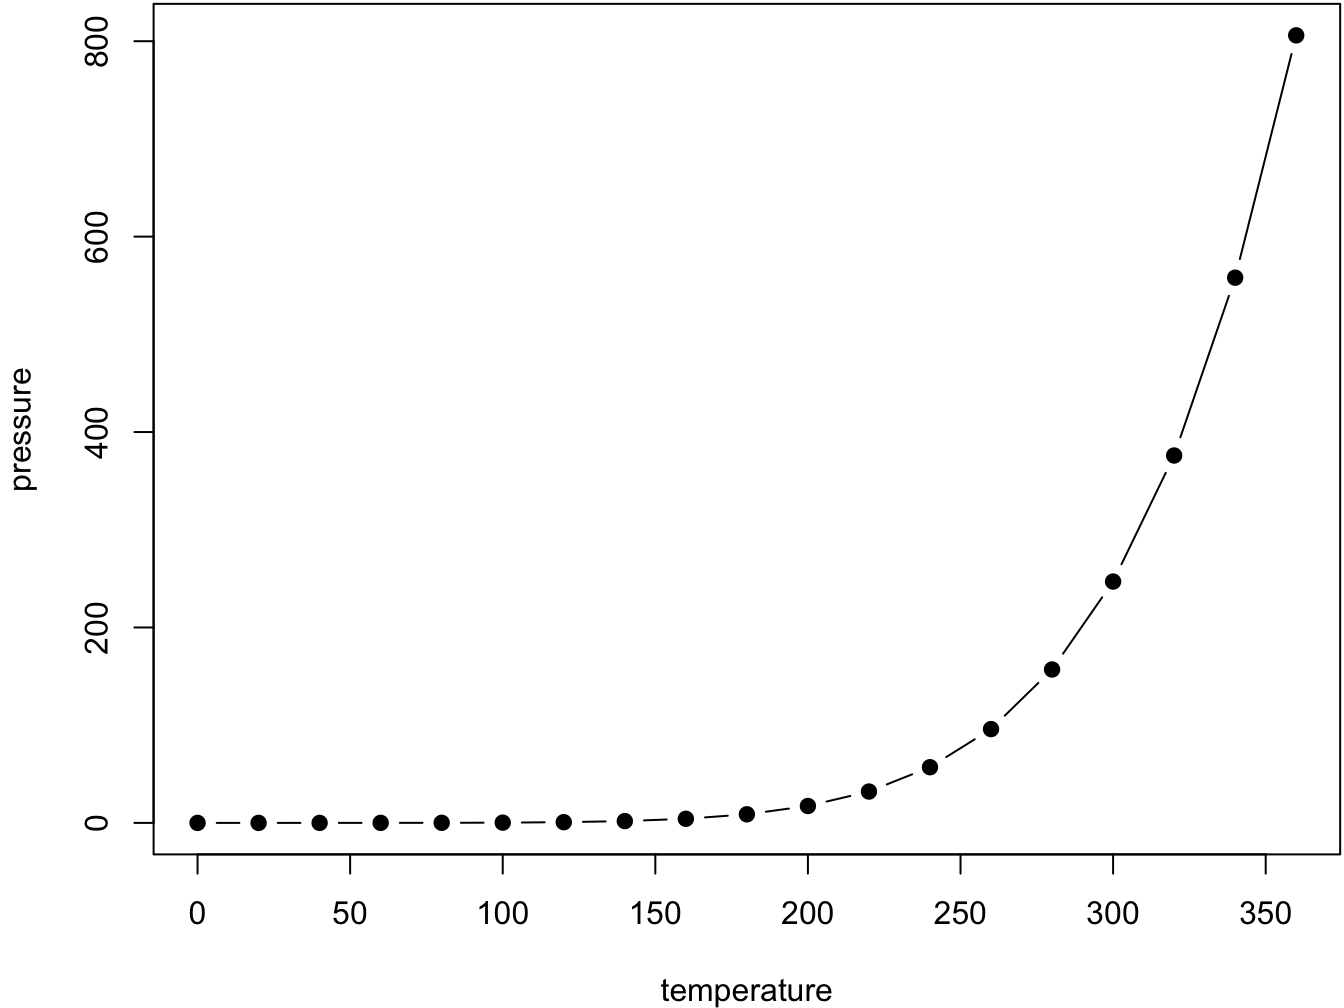
\includegraphics[width=0.8\linewidth]{book_files/figure-latex/nice-fig-1} 

}

\caption{Here is a nice figure!}\label{fig:nice-fig}
\end{figure}

Reference a figure by its code chunk label with the \texttt{fig:} prefix, e.g., see Figure \ref{fig:nice-fig}. Similarly, you can reference tables generated from \texttt{knitr::kable()}, e.g., see Table \ref{tab:nice-tab}.

\begin{Shaded}
\begin{Highlighting}[]
\NormalTok{knitr}\OperatorTok{::}\KeywordTok{kable}\NormalTok{(}
  \KeywordTok{head}\NormalTok{(iris, }\DecValTok{20}\NormalTok{), }\DataTypeTok{caption =} \StringTok{'Here is a nice table!'}\NormalTok{,}
  \DataTypeTok{booktabs =} \OtherTok{TRUE}
\NormalTok{)}
\end{Highlighting}
\end{Shaded}

\begin{table}[t]

\caption{\label{tab:nice-tab}Here is a nice table!}
\centering
\begin{tabular}{rrrrl}
\toprule
Sepal.Length & Sepal.Width & Petal.Length & Petal.Width & Species\\
\midrule
5.1 & 3.5 & 1.4 & 0.2 & setosa\\
4.9 & 3.0 & 1.4 & 0.2 & setosa\\
4.7 & 3.2 & 1.3 & 0.2 & setosa\\
4.6 & 3.1 & 1.5 & 0.2 & setosa\\
5.0 & 3.6 & 1.4 & 0.2 & setosa\\
\addlinespace
5.4 & 3.9 & 1.7 & 0.4 & setosa\\
4.6 & 3.4 & 1.4 & 0.3 & setosa\\
5.0 & 3.4 & 1.5 & 0.2 & setosa\\
4.4 & 2.9 & 1.4 & 0.2 & setosa\\
4.9 & 3.1 & 1.5 & 0.1 & setosa\\
\addlinespace
5.4 & 3.7 & 1.5 & 0.2 & setosa\\
4.8 & 3.4 & 1.6 & 0.2 & setosa\\
4.8 & 3.0 & 1.4 & 0.1 & setosa\\
4.3 & 3.0 & 1.1 & 0.1 & setosa\\
5.8 & 4.0 & 1.2 & 0.2 & setosa\\
\addlinespace
5.7 & 4.4 & 1.5 & 0.4 & setosa\\
5.4 & 3.9 & 1.3 & 0.4 & setosa\\
5.1 & 3.5 & 1.4 & 0.3 & setosa\\
5.7 & 3.8 & 1.7 & 0.3 & setosa\\
5.1 & 3.8 & 1.5 & 0.3 & setosa\\
\bottomrule
\end{tabular}
\end{table}

You can write citations, too. For example, we are using the \textbf{bookdown} package \citep{R-bookdown} in this sample book, which was built on top of R Markdown and \textbf{knitr} \citep{xie2015}.

\hypertarget{advance-design}{%
\chapter{Advance Design}\label{advance-design}}

In this chapter, you will learn how to build your own html templates taken from the web
and package them, so that they can be re-used at any time by anybody.

\hypertarget{selecting-a-good-template}{%
\section{Selecting a good template}\label{selecting-a-good-template}}

There exists tons of HTML templates over the web. However, only a few part will be suitable
for shiny, mainly because of what follows:

\begin{itemize}
\tightlist
\item
  shiny is built on top of \href{https://getbootstrap.com/docs/3.3/}{bootstrap 3} (HTML, CSS and Javascript framework), meaning that going for another framework might
  not be straightforward. However, shinymaterial and shiny.semantic are examples showing
  this can be possible.
\item
  shiny relies on \href{https://jquery.com}{jQuery} (currently v 1.12.4 for shiny, whereas the latest version is 3.3.1). Consequently, all templates based upon React, Vue and other Javascript framework will not be natively supported. Again, there exist some \href{https://github.com/alandipert/react-widget-demo/blob/master/app.R}{examples} for React with shiny and more generally,
  the \href{https://react-r.github.io/reactR/}{reactR} package developed by Kent Russell (\citet{timelyportfolio} on Twitter) and Alan Dipert from RStudio.
\end{itemize}

See \href{https://github.com/rstudio/shiny/tree/master/inst/www/shared}{the github repository} for more details about all dependencies related to the shiny package.

Therefore in the following, we will restict ourself to Bootstrap (3 and 4) together with jQuery. Don't be disapointed since there is still a lot to say.

\begin{quote}
Notes: As shiny depends on Bootstrap 3.3.7, we recommand the user who would like to
experiment Boostrap 4 features to be particularly careful about potential incompatibilies.
See a working example here with \href{https://github.com/RinteRface/bs4Dash}{bs4Dash}.
\end{quote}

A good source of \textbf{open source} HTML templates is \href{https://colorlib.com}{Colorlib} and \href{https://www.creative-tim.com/bootstrap-themes/free}{Creative Tim}. You might also buy your template, but forget about the packaging option, which would be illegal in this particular case, unless you have a legal agreement with the author (very unlikely however).

\hypertarget{about-htmltools}{%
\section{About htmltools}\label{about-htmltools}}

While building a custom html template, you will need to know more about the wonderful \href{https://github.com/rstudio/htmltools}{htmltools} developed by Winston Chang, member of the shiny core team. It has the same spirit as devtools, that is, making your web developer life easier. What follows does not have the pretention to be an exhaustive guide about this package. Yet, it will provide you yith the main
tools to be more efficient.

\hypertarget{html-tags}{%
\subsection{HTML Tags}\label{html-tags}}

Both shiny and htmltools contain tags. However, by experience, htmltools contains more exported tags than shiny.
For instance, the HTML \texttt{\textless{}nav\textgreater{}\textless{}/nav\textgreater{}} tag, namely \texttt{tags\$nav()} in R is not included in the shiny package but
in htmltools.

Within your package code, your tags will be like:

\begin{Shaded}
\begin{Highlighting}[]
\CommentTok{# we use htmltools tags instead of shiny}
\NormalTok{htmltools}\OperatorTok{::}\NormalTok{tags}\OperatorTok{$}\KeywordTok{div}\NormalTok{(...)}
\end{Highlighting}
\end{Shaded}

If you had to gather multiple tags together, prefer \texttt{tagList()} as \texttt{list()}, although the HTML output is the same. The first
has the shiny.tag.list class in addition to list.

\hypertarget{notations}{%
\subsubsection{Notations}\label{notations}}

Whether to use \texttt{tags\$div} or \texttt{div} is the tag is exported by default.
For instance, you could use \texttt{htmltools::div} but not \texttt{htmltools::nav} since nav does not
have a dedicated function (only for p, h1, h2, h3, h4, h5, h6, a, br, div, span, pre, code, img, strong, em, hr).
Rather use \texttt{htmltools::tags\$nav}. Alternatively, there exists a function (in shiny and htmltools)
called \texttt{withTags()}. Wrapping your code in this function enables you to use \texttt{withTags(nav(),\ ...)}
instead of \texttt{tags\$nav()}.

\hypertarget{alternative-way-to-write-tags}{%
\subsubsection{Alternative way to write tags}\label{alternative-way-to-write-tags}}

htmltools and shiny come with the \texttt{HTML()} function that you can feed with raw HTML:

\begin{Shaded}
\begin{Highlighting}[]
\KeywordTok{HTML}\NormalTok{(}\StringTok{'<div>Blabla</div>'}\NormalTok{)}
\CommentTok{# will render exactly like}
\KeywordTok{div}\NormalTok{(}\StringTok{"Blabla"}\NormalTok{)}

\CommentTok{# but there class is different}
\KeywordTok{class}\NormalTok{(}\KeywordTok{HTML}\NormalTok{(}\StringTok{'<div>Blabla</div>'}\NormalTok{))}
\KeywordTok{class}\NormalTok{(}\KeywordTok{div}\NormalTok{(}\StringTok{"Blabla"}\NormalTok{))}
\end{Highlighting}
\end{Shaded}

You will not be able to use tag related functions, as in the following parts.
Therefore, I strongly recommand using R and not mixing HTML in R.

\hypertarget{tags-structure}{%
\subsubsection{Tags structure}\label{tags-structure}}

According to the htmltools \texttt{tag()} function, a tag has:
- a name such as span, div, h1 \ldots{}
- attributes, which you can access with \texttt{tag\$attribs}
- children, which you can access with \texttt{tag\$children}
- a class, namely ``shiny.tag''

For instance:

\begin{Shaded}
\begin{Highlighting}[]
\CommentTok{# create the tag}
\NormalTok{myTag <-}\StringTok{ }\KeywordTok{div}\NormalTok{(}
  \DataTypeTok{class =} \StringTok{"divclass"}\NormalTok{, }
  \DataTypeTok{id =} \StringTok{"first"}\NormalTok{,}
  \KeywordTok{h1}\NormalTok{(}\StringTok{"Here comes your baby"}\NormalTok{),}
  \KeywordTok{span}\NormalTok{(}\DataTypeTok{class =} \StringTok{"child"}\NormalTok{, }\DataTypeTok{id =} \StringTok{"baby"}\NormalTok{, }\StringTok{"Ouinnnnn"}\NormalTok{)}
\NormalTok{)}

\CommentTok{# access its name}
\NormalTok{myTag}\OperatorTok{$}\NormalTok{name}

\CommentTok{# access its attributes (id and class)}
\NormalTok{myTag}\OperatorTok{$}\NormalTok{attribs}

\CommentTok{# access children (returns a list of 2 elements)}
\NormalTok{myTag}\OperatorTok{$}\NormalTok{children}
\end{Highlighting}
\end{Shaded}

How to modify the class of the second child?

\begin{Shaded}
\begin{Highlighting}[]
\NormalTok{second_children <-}\StringTok{ }\NormalTok{myTag}\OperatorTok{$}\NormalTok{children[[}\DecValTok{2}\NormalTok{]]}
\NormalTok{second_children}\OperatorTok{$}\NormalTok{attribs}\OperatorTok{$}\NormalTok{class <-}\StringTok{ "adult"}
\NormalTok{myTag}

\CommentTok{# Hummm, this is not working ...}
\end{Highlighting}
\end{Shaded}

The code above is wrong. Indeed, by assigning \texttt{myTag\$children{[}{[}2{]}{]}} to second\_children,
\texttt{second\_children\$attribs\$class\ \textless{}-\ "adult"} modifies the class of the copy and not the
original object. Only one way:

\begin{Shaded}
\begin{Highlighting}[]
\NormalTok{myTag}\OperatorTok{$}\NormalTok{children[[}\DecValTok{2}\NormalTok{]]}\OperatorTok{$}\NormalTok{attribs}\OperatorTok{$}\NormalTok{class <-}\StringTok{ "adult"}
\NormalTok{myTag}
\end{Highlighting}
\end{Shaded}

For strongly nested tags, you will see that the following section contains amazing functions,
such as \texttt{tagAppenChild()}.

\hypertarget{useful-functions-for-tags}{%
\subsubsection{Useful functions for Tags}\label{useful-functions-for-tags}}

htmltools and shiny have powerful functions to easily add attributes to tags, check for
existing attributes, get attributes and add other tags to a list of tags.

\begin{itemize}
\tightlist
\item
  \texttt{tagAppendAttributes()}: this function allow you to add a new attribute to the current tag.
  For instance, assuming you created a div for which you forgot to add and id attribute:
\end{itemize}

\begin{Shaded}
\begin{Highlighting}[]
\NormalTok{mydiv <-}\StringTok{ }\KeywordTok{div}\NormalTok{(}\StringTok{"Where is my brain"}\NormalTok{)}
\NormalTok{mydiv <-}\StringTok{ }\KeywordTok{tagAppendAttributes}\NormalTok{(mydiv, }\DataTypeTok{id =} \StringTok{"here_it_is"}\NormalTok{)}
\end{Highlighting}
\end{Shaded}

You can pass as many attributes as you want, including non standard attributes such as
\texttt{data-toggle} (see Bootstrap 3 tabs for instance):

\begin{Shaded}
\begin{Highlighting}[]
\NormalTok{mydiv <-}\StringTok{ }\KeywordTok{tagAppendAttributes}\NormalTok{(mydiv, }\StringTok{`}\DataTypeTok{data-toggle}\StringTok{`}\NormalTok{ =}\StringTok{ "tabs"}\NormalTok{)}
\CommentTok{# even though you could proceed as follows}
\NormalTok{mydiv}\OperatorTok{$}\NormalTok{attribs[[}\StringTok{"aria-controls"}\NormalTok{]] <-}\StringTok{ "home"}
\end{Highlighting}
\end{Shaded}

\begin{itemize}
\tightlist
\item
  \texttt{tagHasAttribute()}: to check if a tag has a specific attribute
\end{itemize}

\begin{Shaded}
\begin{Highlighting}[]
\CommentTok{# I want to know if div has a class}
\NormalTok{mydiv <-}\StringTok{ }\KeywordTok{div}\NormalTok{(}\DataTypeTok{class =} \StringTok{"myclass"}\NormalTok{)}
\NormalTok{has_class <-}\StringTok{ }\KeywordTok{tagHasAttribute}\NormalTok{(mydiv, }\StringTok{"class"}\NormalTok{)}
\NormalTok{has_class}

\CommentTok{# if you are familiar with %>%}
\NormalTok{has_class <-}\StringTok{ }\NormalTok{mydiv }\OperatorTok\StringTok{ }\KeywordTok{tagHasAttribute}\NormalTok{(}\StringTok{"class"}\NormalTok{)}
\NormalTok{has_class}
\end{Highlighting}
\end{Shaded}

\begin{itemize}
\tightlist
\item
  \texttt{tagGetAttribute()}: to get the value of the targeted attributes, if it exists, otherwise NULL.
\end{itemize}

\begin{Shaded}
\begin{Highlighting}[]
\NormalTok{mydiv <-}\StringTok{ }\KeywordTok{div}\NormalTok{(}\DataTypeTok{class =} \StringTok{"test"}\NormalTok{)}
\CommentTok{# returns the class}
\KeywordTok{tagGetAttribute}\NormalTok{(mydiv, }\StringTok{"class"}\NormalTok{)}
\CommentTok{# returns NULL}
\KeywordTok{tagGetAttribute}\NormalTok{(mydiv, }\StringTok{"id"}\NormalTok{)}
\end{Highlighting}
\end{Shaded}

\begin{itemize}
\tightlist
\item
  \texttt{tagAppendChild()} and \texttt{tagAppendChildren()}: add other tags to an existing tag.
  Whereas \texttt{tagAppendChild()} only takes on tag, you can pass a list of tags to \texttt{tagAppendChildren()}.
\end{itemize}

\begin{Shaded}
\begin{Highlighting}[]
\NormalTok{mydiv <-}\StringTok{ }\KeywordTok{div}\NormalTok{(}\DataTypeTok{class =} \StringTok{"parent"}\NormalTok{, }\DataTypeTok{id =} \StringTok{"mother"}\NormalTok{, }\StringTok{"Not the mama!!!"}\NormalTok{)}
\NormalTok{otherTag <-}\StringTok{ }\KeywordTok{span}\NormalTok{(}\StringTok{"I am your child"}\NormalTok{)}
\NormalTok{mydiv <-}\StringTok{ }\KeywordTok{tagAppendChild}\NormalTok{(mydiv, otherTag)}
\end{Highlighting}
\end{Shaded}

You might wonder why there is no \texttt{tagRemoveChild()} or \texttt{tagRemoveAttributes()}.

\hypertarget{other-interesting-functions}{%
\subsubsection{Other interesting functions}\label{other-interesting-functions}}

The \href{https://github.com/ThinkR-open/brighter}{brighter} package written by Colin Fay contains
very neat functions to edit your tags. Particularly, the \texttt{tagRemoveAttributes()}

\begin{Shaded}
\begin{Highlighting}[]
\NormalTok{remotes}\OperatorTok{::}\KeywordTok{install_github}\NormalTok{(}\StringTok{"Thinkr-open/brighter"}\NormalTok{)}
\KeywordTok{library}\NormalTok{(brighter)}
\end{Highlighting}
\end{Shaded}

\begin{Shaded}
\begin{Highlighting}[]
\NormalTok{mydiv <-}\StringTok{ }\KeywordTok{div}\NormalTok{(}\DataTypeTok{class =} \StringTok{"test"}\NormalTok{, }\DataTypeTok{id =} \StringTok{"coucou"}\NormalTok{, }\StringTok{"Prout"}\NormalTok{)}
\KeywordTok{tagRemoveAttributes}\NormalTok{(mydiv, }\StringTok{"class"}\NormalTok{, }\StringTok{"id"}\NormalTok{)}
\end{Highlighting}
\end{Shaded}

Up to you to create new functions to add in this package and do a nice PR.

\hypertarget{dependency-utilities}{%
\subsection{Dependency utilities}\label{dependency-utilities}}

When creating a new template, you sometimes need to import custom HTML dependencies
that do not come along with shiny. No problem, htmltools is here for you (shiny also
contains these functions).

\hypertarget{the-dirty-approach}{%
\subsubsection{The dirty approach}\label{the-dirty-approach}}

Let's consider the following example. I want to include a bootstrap 4 card in a shiny app.
This example is taken from an interesting question \href{https://community.rstudio.com/t/create-a-div-using-htmltools-withtags/22439/2}{here}.
The naive approach would be to include the HTML code directly in the app code

\begin{Shaded}
\begin{Highlighting}[]
\KeywordTok{library}\NormalTok{(shiny)}

\CommentTok{# we create the card function before}
\NormalTok{my_card <-}\StringTok{ }\ControlFlowTok{function}\NormalTok{(...) \{}
\NormalTok{  htmltools}\OperatorTok{::}\KeywordTok{withTags}\NormalTok{(}
    \KeywordTok{div}\NormalTok{(}
      \DataTypeTok{class =} \StringTok{"card border-success mb-3"}\NormalTok{,}
      \KeywordTok{div}\NormalTok{(}\DataTypeTok{class =} \StringTok{"card-header bg-transparent border-success"}\NormalTok{),}
      \KeywordTok{div}\NormalTok{(}
        \DataTypeTok{class =} \StringTok{"card-body text-success"}\NormalTok{,}
        \KeywordTok{h3}\NormalTok{(}\DataTypeTok{class =} \StringTok{"card-title"}\NormalTok{, }\StringTok{"title"}\NormalTok{),}
        \KeywordTok{p}\NormalTok{(}\DataTypeTok{class =} \StringTok{"card-text"}\NormalTok{, ...)}
\NormalTok{      ),}
      \KeywordTok{div}\NormalTok{(}\DataTypeTok{class =} \StringTok{"card-footer bg-transparent border-success"}\NormalTok{, }\StringTok{"footer"}\NormalTok{)}
\NormalTok{    )}
\NormalTok{  )}
\NormalTok{\}}

\CommentTok{# we build our app}
\KeywordTok{shinyApp}\NormalTok{(}
    \DataTypeTok{ui =} \KeywordTok{fluidPage}\NormalTok{(}
      \KeywordTok{fluidRow}\NormalTok{(}
       \KeywordTok{column}\NormalTok{(}
        \DataTypeTok{width =} \DecValTok{6}\NormalTok{,}
        \DataTypeTok{align =} \StringTok{"center"}\NormalTok{,}
        \KeywordTok{br}\NormalTok{(),}
        \KeywordTok{my_card}\NormalTok{(}\StringTok{"blablabla. PouetPouet Pouet."}\NormalTok{)}
\NormalTok{       )}
\NormalTok{     )}
\NormalTok{    ),}
    \DataTypeTok{server =} \ControlFlowTok{function}\NormalTok{(input, output) \{\}}
\NormalTok{)}
\end{Highlighting}
\end{Shaded}

and desesperately see that nothing is displayed. If you remember, this was expected since
shiny does not contain bootstrap 4 dependencies and this card is unfortunately a
bootstrap 4 object. Don't panic! We just need to tell shiny to load the css we need to display
this card (if required, we could include the javascript as well). We could use either
\texttt{includeCSS()}, \texttt{tags\$head(tags\$link(rel\ =\ "stylesheet",\ type\ =\ "text/css",\ href\ =\ "custom.css"))}. See
more \href{https://shiny.rstudio.com/articles/css.html}{here}.

\begin{Shaded}
\begin{Highlighting}[]
\KeywordTok{shinyApp}\NormalTok{(}
    \DataTypeTok{ui =} \KeywordTok{fluidPage}\NormalTok{(}
      \CommentTok{# load the css code}
      \KeywordTok{includeCSS}\NormalTok{(}\DataTypeTok{path =} \StringTok{"https://maxcdn.bootstrapcdn.com/bootstrap/4.0.0/css/bootstrap.min.css"}\NormalTok{),}
      \KeywordTok{fluidRow}\NormalTok{(}
       \KeywordTok{column}\NormalTok{(}
        \DataTypeTok{width =} \DecValTok{6}\NormalTok{,}
        \DataTypeTok{align =} \StringTok{"center"}\NormalTok{,}
        \KeywordTok{br}\NormalTok{(),}
        \KeywordTok{my_card}\NormalTok{(}\StringTok{"blablabla. PouetPouet Pouet."}\NormalTok{)}
\NormalTok{       )}
\NormalTok{     )}
\NormalTok{    ),}
    \DataTypeTok{server =} \ControlFlowTok{function}\NormalTok{(input, output) \{\}}
\NormalTok{)}
\end{Highlighting}
\end{Shaded}

The card is ugly (which is another problem we will fix later) but at least displayed.

When I say this approach is dirty, it is because it will not be easily re-usable by others.
Instead, we prefer a packaging approach, like in the next section.

\hypertarget{the-clean-approach}{%
\subsubsection{The clean approach}\label{the-clean-approach}}

We will use the \texttt{htmlDependency} and \texttt{attachDependencies} functions from htmltools.
The htmlDependency takes several arguments:

\begin{itemize}
\tightlist
\item
  the name of your dependency
\item
  the version (useful to remember on which version it is built upon)
\item
  a path to the dependency (can be a CDN or a local folder)
\item
  script and stylesheet to respectively pass css and scripts
\end{itemize}

\begin{Shaded}
\begin{Highlighting}[]
\CommentTok{# handle dependency}
\NormalTok{card_css <-}\StringTok{ "bootstrap.min.css"}
\NormalTok{bs4_card_dep <-}\StringTok{ }\ControlFlowTok{function}\NormalTok{() \{}
\NormalTok{  htmltools}\OperatorTok{::}\KeywordTok{htmlDependency}\NormalTok{(}
    \DataTypeTok{name =} \StringTok{"bs4_card"}\NormalTok{,}
    \DataTypeTok{version =} \StringTok{"1.0"}\NormalTok{,}
    \DataTypeTok{src =} \KeywordTok{c}\NormalTok{(}\DataTypeTok{href =} \StringTok{"https://maxcdn.bootstrapcdn.com/bootstrap/4.0.0/css/"}\NormalTok{),}
    \DataTypeTok{stylesheet =}\NormalTok{ card_css}
\NormalTok{  )}
\NormalTok{\}}
\end{Highlighting}
\end{Shaded}

We create the card tag and give it the bootstrap 4 dependency through the \texttt{attachDependencies()}
function.

\begin{Shaded}
\begin{Highlighting}[]
\CommentTok{# create the card}
\NormalTok{my_card <-}\StringTok{ }\ControlFlowTok{function}\NormalTok{(...) \{}
\NormalTok{  cardTag <-}\StringTok{ }\NormalTok{htmltools}\OperatorTok{::}\KeywordTok{withTags}\NormalTok{(}
    \KeywordTok{div}\NormalTok{(}
      \DataTypeTok{class =} \StringTok{"card border-success mb-3"}\NormalTok{,}
      \KeywordTok{div}\NormalTok{(}\DataTypeTok{class =} \StringTok{"card-header bg-transparent border-success"}\NormalTok{),}
      \KeywordTok{div}\NormalTok{(}
        \DataTypeTok{class =} \StringTok{"card-body text-success"}\NormalTok{,}
        \KeywordTok{h3}\NormalTok{(}\DataTypeTok{class =} \StringTok{"card-title"}\NormalTok{, }\StringTok{"title"}\NormalTok{),}
        \KeywordTok{p}\NormalTok{(}\DataTypeTok{class =} \StringTok{"card-text"}\NormalTok{, ...)}
\NormalTok{      ),}
      \KeywordTok{div}\NormalTok{(}\DataTypeTok{class =} \StringTok{"card-footer bg-transparent border-success"}\NormalTok{, }\StringTok{"footer"}\NormalTok{)}
\NormalTok{    )}
\NormalTok{  )}
  
  \CommentTok{# attach dependencies}
\NormalTok{  htmltools}\OperatorTok{::}\KeywordTok{attachDependencies}\NormalTok{(cardTag, }\KeywordTok{bs4_card_dep}\NormalTok{())}
  
\NormalTok{\}}
\end{Highlighting}
\end{Shaded}

We finally run our app:

\begin{Shaded}
\begin{Highlighting}[]
\CommentTok{# run shiny app }
\NormalTok{ui <-}\StringTok{ }\KeywordTok{fluidPage}\NormalTok{(}
  \DataTypeTok{title =} \StringTok{"Hello Shiny!"}\NormalTok{,}
  \KeywordTok{fluidRow}\NormalTok{(}
    \KeywordTok{column}\NormalTok{(}
      \DataTypeTok{width =} \DecValTok{6}\NormalTok{,}
      \DataTypeTok{align =} \StringTok{"center"}\NormalTok{,}
      \KeywordTok{br}\NormalTok{(),}
      \KeywordTok{my_card}\NormalTok{(}\StringTok{"blablabla. PouetPouet Pouet."}\NormalTok{)}
\NormalTok{    )}
\NormalTok{  )}
\NormalTok{)}

\KeywordTok{shinyApp}\NormalTok{(ui, }\DataTypeTok{server =} \ControlFlowTok{function}\NormalTok{(input, output) \{ \})}
\end{Highlighting}
\end{Shaded}

With this approach, you could develop a package of custom dependencies that people
could use when they need to add custom elements in shiny.

\hypertarget{template-skeleton}{%
\section{Template Skeleton}\label{template-skeleton}}

Now that you have the basis about tags and dependencies, we can go through the template organisation\ldots{}

TO DO

\hypertarget{further-considerations}{%
\section{Further Considerations}\label{further-considerations}}

\bibliography{book.bib,packages.bib}


\end{document}
